\documentclass{llncs}

\usepackage{amsmath}
\usepackage{amsfonts}
\usepackage{listings}
\usepackage[usenames,dvipsnames]{color}
\usepackage{alltt}
\usepackage{xspace}
\usepackage{multirow}
\pagestyle{plain}
\usepackage{xcolor}
\usepackage{algorithm2e}
\usepackage{tikz,pgfplots}
\usepackage{etoolbox}
\usepackage{mathtools}
\usepackage{caption}
%\usepackage{subcaption}
\usepackage{wrapfig}
\usepackage{listings}
%\usepackage{adjustbox}
%\usetikzlibrary{arrows,calc}
\captionsetup{compatibility=false}
%\usepackage{a4wide}
%\usepackage[margin=40mm, top=35mm]{geometry}

%\usepackage{latexsym}
\usepackage{setspace}
\usepackage{cancel}
\usepackage{graphicx}
\usepackage{appendix}
\usepackage{amssymb}
\usepackage{dsfont}
%\usepackage{cancel}
%\usepackage{verbatim}
%\usepackage{chngpage}
%\usepackage{xcolor}
%\usepackage{mathrsfs}


\lstset{language=Java,
	basicstyle=\ttfamily\footnotesize,
	showspaces=false,
	showtabs=false,
	breaklines=true,
	showstringspaces=false,
	breakatwhitespace=true,
	commentstyle=\color{pgreen},
	keywordstyle=\color{blue},
	stringstyle=\color{red},
	basicstyle=\ttfamily
}

\newcommand{\Var}{\mathtt{Var}}
\newcommand{\Exp}{\mathtt{Exp}}
\newcommand{\Cmd}{\mathtt{Cmd}}
\newcommand{\Grd}{\mathtt{Grd}}
\newcommand{\Prg}{\mathtt{Prg}}
\DontPrintSemicolon
\SetKwRepeat{Loop}{Loop\{}{\}}%


\newcommand{\true}{\mathsf{true}}
\newcommand{\false}{\mathsf{false}}

\newcommand{\todo}[1]{{\color{blue}TODO:#1}}
\newcommand{\hide}[1]{}
\newcommand{\defn}{\overset{\triangle}{=}}
\newcommand{\maxi}{m}
\newcommand{\cur}{cur()}
\newcommand{\dom}[1]{\mathsf{dom}(#1)}
\newcommand{\ite}[3]{
	 \ifmmode
	 \mathbf{if}\ #1 \ \mathbf{then}\ #2\  \mathbf{else}\ #3
	 \else
	 \textbf{if}\ #1 \ \textbf{then}\ #2\  \textbf{else}\ #3
	 \fi}
\newcommand{\rloop}{
	\ifmmode
	\mathbf{Loop}
	\else
	\textbf{Loop}
	\fi}

\newcommand{\Z}{\mathbb{Z}}

\title{J-ReCoVer: Java Reducer Commutativity Verifier}

\author{
Yu-Fang Chen\inst{1}\inst{2}
\and
Chang-Yi Chiang\inst{2}
\and
Hung-Wei Hsu\inst{1}
\and
Wei-Tsung Kao\inst{1}
\and
Yen-Fu Wen\inst{2}
\and
Wei-Cheng Wu\inst{1}
}
\institute
{
Institute of Information Science, Academia Sinica, Taiwan
\and
Graduate Institute of Information Management, National Taipei University, Taiwan
}

\begin{document}


\maketitle

\begin{abstract}

MapReduce framework for data-parallel computation was first proposed by Google~\cite{dean04} and later implemented in the Apache Hadoop project~\cite{hadoop}.
Under the MapReduce framework, the reducer computes output values from a sequence of input values transmitted over the network.  Due to the non-determinism in data transmission, the order of input values arrived at the reducer is not fixed.
The \emph{commutativity problem} of reducers asks if the output of a reducer is independent of the order of its inputs. There are several advantages for a reducer being commutative, e.g., the verification problem of a MapReduce program can be reduced to the problem of verifying a sequential program. 
In this paper, we propose effective heuristics for reducer commutative analysis and implement them as a tool J-ReCoVer (Java Reducer Commutativity Verifier), which is the first tool that is specialized in checking reducer commutativity. Experimental results over 128 benchmark examples collected from literature and open repositories are very positive; J-ReCoVer correctly handles over 97\% of them.

\end{abstract}

\section{Introduction}
\label{section:introduction}

MapReduce is one of the most popular framework for data parallel computation.
A MapReduce~\cite{dean04,hadoop} program consists of several pairs of \emph{mappers} and \emph{reducers} running on a machine cluster for handling big data in parallel. Usually mappers and reducers are the only components in a MapReduce program that involves concurrency. Mappers read data from a distributed database and output a sequence of \emph{key-value} pairs. The sequence elements (key-value pairs) with the same key will be sent to the same reducer for further processing. Due to scheduling polices and network latency, the same inputs may arrive at a reducer in different order in different executions, which results in the so-called \emph{commutativity problem} of reducers~\cite{csallner13testing,xiao14mr,ChenHSW15,ChenSW16}, that is, if the outputs of a reducer is independent of the order of its inputs. 
If all reducers are commutative, they will have the same external behavior under all possible schedules. In such a case, by fixing a schedule, the verification problem of a MapReduce program can be reduced to the verification problem of a sequential program, which is known to be much easier then the verification problem of concurrent programs. One needs to consider only a particular interleaving of input values instead of all of them.


\hide{More concretely, for the verification of a MapReduce program, we propose to do it in two phases. First, ensuring if all reducers are commutative. If some reducers are non-commutative, modifying them to commutative ones. Usually, the modification is not a difficult task~\cite{xiao14mr}, and can be done without affecting their functionality and performance. For example, assume that the task of a reducer is to find the name of the person with highest score. Such a reducer is non-commutative when the input include two people with the same highest score. This reducer can be made commutative, by also comparing the ID number of people with the same score. Once all reducers are made commutative, we reduce the verification problem to sequential verification by fixing a scheduler. In this two-phase approach, the key enabling technique is an efficient procedure for checking reducer commutativity.}

On the other hand, in many cases, the non-commutative behavior of a reducer can be the source of very tricky bugs. A study conducted by Microsoft investigated the commutativity problem of $508$ reducers running on their MapReduce server~\cite{xiao14mr}. The reducer programs have been checked carefully using all traditional means such as code review, testing, and experiments with real data for months. Still, among them, five programs contain very subtle bugs caused by non-commutativity (confirmed by the programmers).

However, checking reducer commutativity is a difficult problem on its own right~\cite{ChenHSW15,ChenSW16,ChenLTW17}. Even for a simple case that all values are mathematical integers, it is proved undecidable in~\cite{ChenHSW15}. For the case that all values are machine integer (e.g, 64-bits integer), the problem is decidable, but the only available algorithm that was proposed in the same paper is of very high complexity and hence is only of theoretical interests.

In this paper, we propose heuristics for the commutativity problem that works very efficiently on a large set of practical integer reducer programs. We reduce the commutativity problem to a SMT problem in a sounds but incomplete manner; it  reports commutative only when it holds for all possible initial valuations, even if some of them are in fact unreachable. We also propose optimizations to enable the approach working on real world examples. For the case that the reducer is not proven commutative, we complement the approach by using testing to find concrete counterexamples. We implement those heuristics as a tool called J-ReCoVer (Java Reducer Commutativity Verifier), which is available at~\verb|http://jrecover.iis.sinica.edu.tw|.

We use two sets of integer reducer benchmarks to evaluate J-ReCoVer. The first set is collected from open repositories such as Github and Bitbuckect. With the help of a search engine~\cite{searchcode} over those repositories, we collected 118 examples. J-ReCoVer is able to correctly analyze all but 3 of them. We also tried all 10 integer reducers descried in verification literature~\cite{ChenHSW15,ChenSW16} and J-ReCoVer can handle all of them.


\subsection*{Related Works}
Reducer commutativity problem can be reduced to program equivalence problem. One creates another program $R'$ that first non-deterministically swaps two consecutive input values and then executes the code of $R$. If $R'$ and $R$ are equivalent, using the fact that all permutations of a list can be obtained by swapping consecutive list elements finitely many times\footnote{Here is an example to produce [3;2;5;1;4] from [1;2;3;4;5] by swapping consecutive elements: [\textbf{1};\textbf{2};3;4;5] $\rightarrow$ [2;\textbf{1};\textbf{3};4;5] $\rightarrow$ [2;3;1;\textbf{4};\textbf{5}]$\rightarrow$ [2;3;\textbf{1};\textbf{5};4]$\rightarrow$ [\textbf{2};\textbf{3};5;1;4]$\rightarrow$ [3;2;5;1;4].}, $R$ can be proved to be commutative. There are a series of research results on program equivalence checking (or closely related topics such as regression verification)~\cite{symdiff,fedyukovich2015automated,sharma2013data,godlin2009regression,fedyukovich2016property,felsing2014automating,KieferKlebanovUlbrich2017,lahiri2013differential,grossman2017verifying,barthe2011relational,KlebanovRuemmerUlbrich2017}. At a high level, checking equivalence of two programs $P$ and $P'$ can be reduced to a sequential verification problem by executing $P'$ after $P$ and at the end checking if they always have the same outputs. It can be made more efficient by finding the right~\emph{synchronization points} and combining the code of $P$ and $P'$ in an interleaved manner. A lot of the research effort in this research direction is in finding good synchronization points. For the case of commutativity analysis, good synchronization points are already given; one can simply use the beginning of the loop as the synchronization point. However, in our experience, if we naively reduce the commutativity problem to equivalence problem and check it in a precise manner, many examples cannot be solved. In this paper, we propose a good over-approximation (c.f. Section~\ref{sec:prover}) of the reducer's behavior. The approximation allows a much more efficient yet precise enough commutativity analysis.

One main motivation of commutativity analysis is to reduce verification problem of a concurrent program to a sequential one. There are several researches sharing the similar motivation. For instance, the concept of \emph{robustness} of event-driven asynchronous programs~\cite{ahmed2017:robustness}  and program running under relaxed memory model~\cite{ahmed2013:robustness,AbdullaACLR13,AbdullaACLR12}, \emph{synchronizability} of communicating finite state machines~\cite{FinkelL17,basu2012synchronizability,basu2011choreography}. However, their computation models are quite different to that of reducers and hence the result cannot be directly applied. Besides verification, another interesting research direction is the synthesis of MapReduce programs~\cite{SmithA16}. Commutativity analysis is used as a component under the synthesis framework.

\section{Notations and Definitions}
\label{section:integer-reducers}
We use $\Z$ to denote the set of integers and $[n,m]$ to denote the set of integers $\{k\mid n \leq k\leq m\}$. 
We lift the equality $=$ operation to tuples in the standard way.
Let $S\subseteq [1,k]$, the equality $\{v_1,\ldots,v_k\}=_{S} \{v'_1,\ldots,v'_k\}$ between tuples holds if and only if $\bigwedge_{i\in S} v_i=v'_i$.
For presentation purpose, we describe a highly simplified model to characterize the essence of reducers. The model allows to describe the computation of reducers and investigate their commutativity.

\begin{equation*}
\begin{array}{rclcl}
\multicolumn{3}{l}{v\in \Var\mbox{, and }c \in \Z}&&\textmd{Variable and Constant}\\
e \in \Exp    &\ \ \  {\triangleq}\ \ \   & v \mid c \mid \cur \mid e + e \mid e - e \mid e \times e \mid *\mid\ldots & &\textmd{Integer Expression}\\
g\in \Grd  & {\triangleq}  & e < e \mid not\ g \mid g \wedge g  \mid \ldots& & \textmd{Guard}\\
s\in \Cmd  & {\triangleq}  & v:= e \mid out(v) \mid \ite{g}{s}{s} \mid s;s && \textmd{Command}\\
p\in \Prg  & {\triangleq}  & s.\rloop\{s\}.s&& \textmd{Reducer Program}\\
\end{array}
\end{equation*}

Here $v\in \Var$ and $c \in \Z$ are variables and constant integer values, respectively. An \emph{integer expression} in $\Exp$ can be either a variable, constant value, a call to the $\cur$ function that reads and consumes an input value of the reducer, their combinations over basic arithmetic operations, or a non-deterministically chosen integer value $*$.
A \emph{guard} in $\Grd$ can be a comparison between two expressions or boolean combinations of several guards. A \emph{command} in $\Cmd$ can be an assignment, a branch statement, concatenation of a sequence of commands, or $out(v)$ that outputs the value of $v$.
A \emph{reducer program} is defined as $s_1;\rloop\{s_2\};s_3$, where $s_1,s_2,s_3 \in \Cmd$, and $s_2$ is assumed to have at most one $\cur$ expression in each branch\footnote{We define a \emph{branch} of a command $s$ as a sequence obtained by replacing every branch statement $\ite{g}{s_1}{s_2}$ in $s$ with either $(g)\wedge s_1$ or $(not\ g) \wedge s_2$.} . According to our observation over hundreds  of reducer programs in open repositories, reducer programs are almost always in this form. The $\rloop\{s_2\}$ statement enters the loop body to execute $s_2$ repeatedly until the entire input list is consumed. A few examples of reducer programs in this model can be found in Figure~\ref{fig:reducer_example}. 


Some reducer uses two loops to compute the output. For example, for calculating standard deviation, one first computes the average of inputs and then uses it to compute the standard deviation. In that case, we can still verify the reducer by first partitioning it into two reducers and then verifying them separately. One reducer computes the average (Figure~\ref{fig:reducer_example}(b)) and the other reducer uses a non-deterministic value to over-approximate the computed average ($a := *$) and then use it in the computation of standard deviation (Figure~\ref{fig:reducer_example}(c)). The reducer in Figure~\ref{fig:reducer_example}(c) ``over-approximates''  all possible output of the standard deviation computation; it computes an output even if $a$ is not the average of inputs. However, the reducer is still commutative and its commutativity verification can still be done.


\begin{figure}
	\begin{minipage}{0.32\textwidth}
		\begin{algorithm}[H]
			$m := \cur$; \;
			\Loop{}{
				$t:=\cur$;\;
				\uIf{ $t > m$}{
					$m := t$
				}
			};
			$out(m)$\;
		\end{algorithm}
		\caption*{(a) max}
	\end{minipage}
	\hspace{-0.5cm}
	\begin{minipage}{0.3\textwidth}
		\begin{algorithm}[H]
			$s := 0;c:=0$; \;
			\Loop{}{
				$s := s+\cur$;\;
				$c := c+1$
			};
			$o := s/c$;\;
			$out(o)$\;
		\end{algorithm}
		\caption*{(b) average}
	\end{minipage}
	\begin{minipage}{0.4\textwidth}
		\begin{algorithm}[H]
			$a:=*;s := 0; c:=0$;\;
			\Loop{}{
				$s := s+(\cur-a)^2$; \;
				$c := c+1$
			};
			$o := s/c$;\;
			$out(o)$
		\end{algorithm}
		\caption*{(c) standard deviation}
	\end{minipage}	
	\caption{Example of reducer programs}
	\label{fig:reducer_example}
\end{figure}

In the next section, we give a brief overview of J-Recover,  our tool for reducer commutativity verification.

\section{Overview of the J-ReCoVer tool}
\label{sec:overview}
%Hadoop, Java;
The input of J-ReCoVer is a reducer program written in Java, which is the most popular programming language used in the Hadoop~\cite{hadoop} MapReduce framework. 
The J-ReCoVer tool has three main components, the \emph{Preprocessor}, the \emph{Prover}, and the \emph{BugFinder}. As the name suggests, the Preprocessor reads as input a reducer program and performs the required preprocessing.  The goal of Prover is to show that a given reducer is commutative and the goal of BugFinder is the opposite. The architecture of J-ReCoVer can be found in Figure~\ref{fig:overview-jrecover}. The user can input a reducer program to J-ReCoVer either through our web-interface or binary installed on their own machine. 

\begin{figure}[h]

	\scalebox{0.9}{
		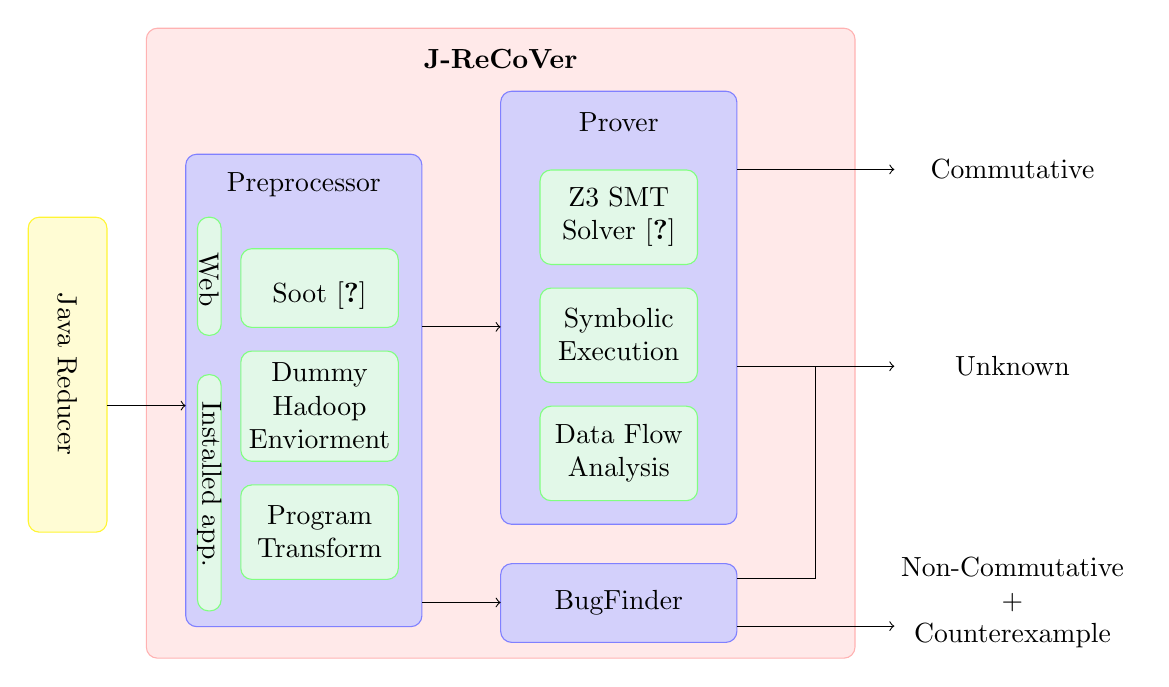
\begin{tikzpicture}


		%J-ReCoVer
		\node[draw=red!30, inner sep=0, anchor=north,rounded corners, fill opacity=0.85,text width=9cm,fill=red!10,minimum height=8cm] (jrecover) at (5.5,0.8) {};
		\node at (5.5,0.4) {\textbf{J-ReCoVer}};

		%JAVA reducer
		\node[draw=yellow!80, inner sep=0, anchor=north,rounded corners, fill opacity=0.85,text width=1cm,fill=yellow!20,minimum height=4cm] (reducer) at (0,-1.6) {};
		\node[rotate=270, align = center] at (0,-3.6) {Java Reducer};


		%JPreprocessor
		\node[draw=blue!50, inner sep=0, anchor=north,rounded corners, fill opacity=0.85,text width=3cm,fill=blue!20,minimum height=6.cm] (preprocessor) at (3,-.8) {};
		\node[] at (3,-1.2) {Preprocessor};

		%JPreprocessor->Interface
		\node[draw=green!50, inner sep=0, anchor=north,rounded corners, fill opacity=0.85,text width=0.3cm,fill=green!10,minimum height=1.5cm] (interface1) at (1.8,-1.6) {};
		\node[rotate=270, align = center] at (1.8,-2.4) {Web};

		\node[draw=green!50, inner sep=0, anchor=north,rounded corners, fill opacity=0.85,text width=0.3cm,fill=green!10,minimum height=3cm] (interace2) at (1.8,-3.6) {};
		\node[rotate=270, align = center] at (1.8,-5) {Installed app.};

		%JPreprocessor->Technologies
		\node[draw=green!50, inner sep=0, anchor=north,rounded corners, fill opacity=0.85,text width=2cm,fill=green!10,minimum height=1cm] (soot) at (3.2,-2) {};
		\node at (3.2,-2.6) {Soot~\cite{soot}};

		\node[draw=green!50, inner sep=0, anchor=north,rounded corners, fill opacity=0.85,text width=2cm,fill=green!10,minimum height=1.4cm] (symex) at (3.2,-3.3) {};
		\node at (3.2,-4) {
			\begin{minipage}[t]{0.222\textwidth}
			\centering
			Dummy\\
			Hadoop\\
			Enviorment
			\end{minipage}
			};

			\node[draw=green!50, inner sep=0, anchor=north,rounded corners, fill opacity=0.85,text width=2cm,fill=green!10,minimum height=1.2cm] (prog_trans) at (3.2,-5) {};
			\node at (3.2,-5.6) {
				\begin{minipage}[t]{0.222\textwidth}
				\centering
				Program\\
				Transform
				\end{minipage}
			};

		%JProver
		\node[draw=blue!50, inner sep=0, anchor=north,rounded corners, fill opacity=0.85,text width=3cm,fill=blue!20,minimum height=5.5cm] (prover) at (7,0) {};
		\node[] at (7,-0.4) {Prover};

		%JProver->Technologies
		\node[draw=green!50, inner sep=0, anchor=north,rounded corners, fill opacity=0.85,text width=2cm,fill=green!10,minimum height=1.2cm] (z3) at (7,-1) {};

		\node at (7,-1.6) {
			\begin{minipage}[t]{0.222\textwidth}
			\centering
			Z3 SMT \\
			Solver~\cite{z3}
			\end{minipage}
		};

		\node[draw=green!50, inner sep=0, anchor=north,rounded corners, fill opacity=0.85,text width=2cm,fill=green!10,minimum height=1.2cm] (z3) at (7,-2.5) {};

		\node at (7,-3.1) {
			\begin{minipage}[t]{0.222\textwidth}
			\centering
			Symbolic \\
			Execution
			\end{minipage}
		};

		\node[draw=green!50, inner sep=0, anchor=north,rounded corners, fill opacity=0.85,text width=2cm,fill=green!10,minimum height=1.2cm] (z3) at (7,-4.) {};

		\node at (7,-4.6) {
			\begin{minipage}[t]{0.222\textwidth}
			\centering
			Data Flow \\
			Analysis
			\end{minipage}
		};

		%JBugFinder
		\node[draw=blue!50, inner sep=0, anchor=north,rounded corners, fill opacity=0.85,text width=3cm,fill=blue!20,minimum height=1cm] (learner) at (7,-6) {};
		\node[] at (7,-6.5) {BugFinder};


		%JResults

		\node at (12,-1) {
			Commutative
		};

		\node at (12,-3.5) {
			Unknown
		};

		\node at (12,-6.5) {
			\begin{minipage}[t]{0.25\textwidth}
			\centering
			Non-Commutative	 \\
			+\\
			Counterexample
			\end{minipage}

		};


		\draw [->] (8.5,-6.8) -- (10.5,-6.8) ;
		\draw [->] (8.5,-1) -- (10.5,-1) ;
		\draw [-] (8.5,-6.2) -- (9.5,-6.2) --(9.5,-3.5);
		\draw [->] (8.5,-3.5) -- (10.5,-3.5) ;

		\draw [->] (4.5,-3) -- (5.5,-3) ;
		\draw [->] (4.5,-6.5) -- (5.5,-6.5) ;

		\draw [->] (0.5,-4) -- (1.5,-4) ;

		\end{tikzpicture}
	}
	\caption{Overview of the J-ReCoVer Tool. }\label{fig:overview-jrecover}
\end{figure}


\textbf{The Preprocessor component} first compiles a reducer program to bytecode and use the tool Soot~\cite{soot} to further convert it to the so called ``Jimple'' format, which is an intermediate language that is designed to simplift the analysis of Java programs. Under the Hadoop MapReduce framework, the permutation of the input is handled by the scheduler/shuffler component and is affected by things like network latency, which is not controllable by programmers. In order to deal with this issue, we wrote our own dummy Hadoop environment for the reducer as a part of the Preprocessor component. So that the input order of the reducer is now controlled by J-ReCoVer. Finally, we perform in the Preprocessor some simple program transformations tasks to simplify the analysis. For example, we convert all output commands $out(e)$ inside loops to an special assignment (Section~\ref{sec:program_trans1} and~\ref{sec:program_trans2}).

\textbf{The BugFinder component} randomly generated 1500 pairs of lists. The lists in a pair are permutations of each other. A concrete counterexample is reported if inputting any pair of lists from the 1500 generated ones to the reducer generates different results.
Our procedure for generating random pairs is quite naive. We use five different input list of lengths 5, 7, 9 ,11, and 13. For each length, we generate 300 lists and pick uniformly at random one of its permutations. Although the approach is simple, in practice it finds counterexamples in all of our non-commutative benchmarks.

\textbf{The Prover component} reduces the commutativity problem to a SMT formula satisfiability problem. At a high level, we check equivalence between a reducer program and its variant that have two consecutive inputs swapped. We show that this can be reduced to a SMT problem and give it to SMT solver Z3~\cite{z3} for solving. Recall that all permutations of a list can be obtained by swapping consecutive elements finitely many times. In case that Z3 proved the formula unsatisfiable, we know that swapping any two consecutive inputs of the reducer will not change its output. It follows that the reducer outputs the same value for all permutations of the same list of input.
In this case,  J-ReCoVer stops and reports that the reducer is commutative. 
If we run the approach in a naive manner, it does not scale to large programs and is very imprecise.  We will introduce two critical optimizations that enables the proposed approach working for real-world examples in Section~\ref{section:optimizations}: a data flow analysis to extract critical variables and an improved symbolic execution algorithm to generate Z3 formulae. More details of the algorithms used in the Preprocessor and the Prover components will be explained in Section~\ref{sec:preprocessor_prover} and the optimizations will be introduced in~\ref{section:optimizations}. 




\section{The Preprocessor and the Prover}
\label{sec:preprocessor_prover}

Before entering the Prover component, the Preprocessor first performs a few program transformation tasks to simplify the verification task.
We assume the reducer $s_1;\rloop\{s_2\};s_3$ is given. We begin the section with our first program transformation task (Section~\ref{sec:program_trans1}) that handles the case when $s_2$ contains $out$ commands. The output of the first transformation task is a commutativity-equivalent reducer program where $out$ does not occur in $s_2$.  Then we explain the algorithm of the Prover (Section~\ref{sec:prover}) that works only in a special case where no read from input occurs in $s_1$. For general reducer programs, we introduce the second program transformation task (Section~\ref{sec:program_trans2}) whose output is a reducer program that contains all input/output behaviors of the original reducer (may contain behaviors that are not in the original reducer) and there is no read from input (i,e., does not have the $\cur$ expression) in $s_1$, which can be analyzed by the algorithm of Prover.

\subsection{The First Program Transformation Task in the Preprocessor}
\label{sec:program_trans1}
J-ReCoVer  first generates a new variable $v_{out_k}$ for the $k$-th output command $out(e)$ inside $s_2$ and replace the $out(e)$ command with an assignment $v_{out_k}:=e$. 
Notice that the value of $v_{out_k}$ stays the same from the point it has been assigned a value. 
If the values of $v_{out_k}$ are the same for all permutations of input lists at the end of $s_2$, we know that the reducer is commutative w.r.t. to all output values produced inside the loop body $s_2$.

\subsection{The Prover: Reducing Commutativity to SMT Solving}
\label{sec:prover}
Below we begin with a simple version where $s_1$ never calls the $\cur$ function. Later we will explain how to handle the general case using program transformation. The command $s_2$ can be viewed as a function $F$ that reads the values of all variables and the current input before executing $s_2$ and outputs values of all variables after $s_2$. Formally, the function $F(n,x_1,x_2,\ldots,x_k): \Z^{k+1} \rightarrow \Z^k$ returns a tuple of values $x_1',x_2',\ldots,x_k'$, where $k$ is the current input value of the reducer, $x_i$ and $x_i'$ are the values of variables before and after the execution of $s_2$, respectively. The construction of $F$ from $s_2$ can be done in the standard way. We will introduce a more efficient data structure for the construction in Section~\ref{section:optimizations}.

We check if the formula below is valid for all possible values of $n_1,n_2, x_1,x_2,\ldots,x_k$. 
\begin{equation}
 F(n_1, F(n_2,x_1,x_2,\ldots,x_k)) = F(n_2, F(n_1,x_1,x_2,\ldots,x_k) )
\label{eq:commu}
\end{equation}

Using the reducer that computes average (Figure~\ref{fig:reducer_example} (b)) as an example. It has two variables $s$ and $c$. It is not difficult to compute that $F_{average}(n,s,c)=(s+n, c+1)$. In this case, the corresponding Equation~(\ref{eq:commu}) is valid because $F_{average}(n_1, F_{average}(n_2,s,c)) =F_{average}(n_1, s+n_2, c+1)= (s+n_1+n_2,c+2)=F_{average}(n_2, s+n_1, c+1)=F_{average}(n_2, F_{average}(n_1,s,c))$.

The validity of Equation~(\ref{eq:commu}) implies that swapping any two consecutive input values does not change the final variable valuation. Informally, it says that starting from the same initial valuations of variables and with two different input orders, the values of all program variables are the same after we execute the loop body twice. The first execution reads $n_1$ and then reads $n_2$. The other execution reads the two inputs in the reverse order.

In the example of ``average'', the values of $s$ and $c$ are the same no matter the reducer first reads $n_1$ and then $n_2$ or reads the two values in the swapped order.
So it computes the same value for the input [1;2;3;4;5] and any other input with two consecutive values swaps, e.g., [1;2;\textbf{4};\textbf{3};5].
Since any permutation of a sequence can be obtained by swapping consecutive values finitely many times~\cite{algebra}, this further implies that starting from the same variable valuation, the loop ends with the same valuation for any permutation of input values, e.g., the reducer will output the same value for [1;2;\textbf{3};\textbf{4};5], [1;\textbf{2};\textbf{4};3;5], [\textbf{1};\textbf{4};2;3;5], [4;1;2;3;5], etc. 
Recall that the first program transformation task remembers all output values in variables that will stay unchanged until the end of the loop. The validity of Equation~(\ref{eq:commu}) also implies that the execution of the loop produces the same sequence of outputs.

We explain why that the validity of Equation~(\ref{eq:commu}) is sufficient to prove the commutativity of the reducer $s_1;\rloop\{s_2\};s_3$. Notice that $s_1$ does not read from the input (assumed at the beginning of this subsection). The execution of $s_1$ is deterministic in the sense that from the same initial valuation, it outputs the same sequence of values and ends at the same valuation. For the execution of $\rloop\{s_2\}$, from the validity of Equation~(\ref{eq:commu}), any permutation of input values leads the reducer to the same final valuation and the same sequence of outputs at the end of the loop. 
Before executing the commands after the loop $s_3$, all inputs have been read (the loop exit condition) already, similar the case of $s_1$, the execution of $s_3$ is deterministic for all permutations of inputs and outputs the same sequence of values. 

In the next subsection, we explain how to generalize our approach to support general reducer programs using program transformation.

\subsection{The Second Program Transformation Task in the Preprocessor}
\label{sec:program_trans2}


\begin{figure}[t]
	\begin{minipage}{0.4\textwidth}
		\begin{algorithm}[H]
			\;\;$m := \cur + 10$; \;
			\Loop{}{
				$t:=\cur$\;
				\uIf{ $t> m$}{
					$m := t$ \;
				}
			};
			$out(m)$\;\;
		\end{algorithm}
		\caption*{(a) Reducer max$^+$}
	\end{minipage}
		\begin{minipage}{0.6\textwidth}
			\begin{algorithm}[H]
				$s:=*;$\;
				\Loop{}{
					\uIf{$s=1$}{$m := \cur + 10; s:= 2$}
					\uElse{
						$t:=\cur$\;
						\uIf{ $t > m$}{
							$m := t$ \;
						}
					}
				};
				$out(m)$
			\end{algorithm}
			\caption*{(b) Reducer max$^{+\mathtt{fix}}$}
		\end{minipage}
	\caption{Reducer examples}
	\label{fig:reducer_max}
\end{figure}





In real-world examples, it is often that the $s_1$ part of the reducer also reads from the input. In the example in Figure~\ref{fig:reducer_max} (a), the reducer program remembers the first input value in the variable $m$, increases its value by 10, and then updates its value to bigger ones if any occurs in the loop. The corresponding Equation~(\ref{eq:commu}) is valid in this case. However, the reducer is not commutative. A counterexample can be easily found. With the list $[1,2,3,4,5]$ and its permutation $[5,4,3,2,1]$ as the inputs, the reducer respectively outputs $11$ and $15$. 

We handle the problem again by program transformation. To handle the example in Figure~\ref{fig:reducer_max} (a), we move the prefix $s_1$ into the loop body and use a new variable $s$ to force that $s_1$ is always executed before the original loop body. The result after the transformation is demonstrated in Figure~\ref{fig:reducer_max} (b). Observe that the new reducer program over-approximates all possible inputs/outputs of the original one.
It also satisfies all assumptions required for the Prover component: (a) The commands before entering the loop does not have any $\cur$ expression and (II) each branch (recall that ``branch'' is formally defined in Section~\ref{section:integer-reducers}) of the loop body has at most one $\cur$. So we can apply Equation~(\ref{eq:commu}) to prove its commutativity.

Since the new reducer has all the possible outputs of the original one, the new reducer being commutative implies that the original one is also commutative. 

\begin{figure}[htb]
	\centering
	\begin{minipage}{0.8\textwidth}

	\begin{algorithm}[H]
		$s'_0;s:=*;$\;
		\Loop{}{
			\lIf{$s=1$}{ $x_{i_1} := \cur; s'_1; s:=2$}
			\lElseIf{ $s =2$}{ $x_{i_2} := \cur; s'_2; s:=3$}
			\lElseIf{ $s = 3$}{$\ldots$}
			\lElseIf{ $s = m$}{$x_{i_m} := \cur; s'_m; s:=m+1$}
			\lElse{ $s_2$}
		};$s_3$\;
	\end{algorithm}
	\end{minipage}
	\caption{The second transformation task}
	\label{fig:general_program_transformation}
\end{figure} 


For the general case, we first rewrite the $s_1$ part of the reducer $s_1;\rloop\{s_2\};s_3$ to the form 
$$s'_0;x_{i_1}{:=} \cur;s'_1.\ldots x_{i_{m}}{:=}\cur;s'_m, $$ where $\cur$ never occur in $s'_0,s'_1,\ldots, s'_m$. Then we produce the reducer in Figure~\ref{fig:general_program_transformation}, which is an over-approximation of the original reducer. For the case that $s=1$ at the beginning, its output sequence is the same as the original reducer. When $s\neq 1$, it may produce outputs that are not possible by the original reducer. Observe that the reducer in Figure~\ref{fig:general_program_transformation} satisfies all assumptions required for the Prover: each branch has at most one $\cur$. Hence the Equation~(\ref{eq:commu}) can then be applied to prove its commutativity.


\section{Optimizations}
\label{section:optimizations}
In this section we explain how data flow analysis are used in J-Recover to improve the precision of commutativity checking and the algorithm we used to construct the $F$ function in Equation~(\ref{eq:commu}).

\subsection{Improving the precision of commutativity verification using data flow analysis}
\label{section:opt1}
We find that in many cases, Equation~(\ref{eq:commu}) is a condition that is too strong for the reducer to be commutative. For instance, consider the example in Figure~\ref{fig:reducer_opt}, in the loop body, the input is first stored in a variable $t$ and then added to $s$. In this case, the $F$ function returns the updated values of both $s$ and $t$ after the execution of loop body. Observe that 
$F(c_1, F(c_2,s,t) = (c_1+c_2, c_1)$ and $F(c_2, F(c_1,s,t) = (c_1+c_2, c_2)$. It follows that the corresponding Equation~(\ref{eq:commu}) is invalid. The second component of the returned tuple, which corresponds to the value of $t$ after executing the loop body twice, are $c_1$ and $c_2$, respectively. However, in this case, the value of $t$ is not important to the output of this reducer. 


\begin{figure}[hbt]
	\begin{minipage}{0.4\textwidth}
		\begin{algorithm}[H]
			$s:= 0$; \;
			\Loop{}{
				$t:=\cur$;
				$s:= s + t$\;
			};
			$out(s)$\;\;
		\end{algorithm}
		\caption{A commutative reducer with an invalid Equation~(\ref{eq:commu}).}
		\label{fig:reducer_opt}
	\end{minipage}
	\begin{minipage}{0.55\textwidth}
		\LinesNumbered
		\centering
		\begin{minipage}{0.75\textwidth}
		\begin{algorithm}[H]
			$c_1;c_2;\ldots;c_i$\;
			\lIf{$g_1$}{$\ldots$}
			\lElseIf{ $g_2$}{$\ldots$}
			\lElseIf{ $g_3$}{$\ldots$}
			\lElseIf{ $g_m$}{$c_{i+1};\ldots ;c_n; out(v);\ldots$}
			\lElse{ $\ldots$}
		\end{algorithm}
	\end{minipage}
		\caption{$out(v)$ in nested branches of $s_3$.}
		\label{fig:nested_out}
	\end{minipage}
\end{figure}


To handle such a situation, we perform a simple backward data flow analysis to collect all variables whose value may propagate to the output command after the loop execution. With out loss of generality, we assume there is only one output command after the loop. Then the code after the loop (i.e., the $s_3$ part of the reducer) can only be in the form of Figure~\ref{fig:nested_out}.
We unfold all concatenation of commands, so now the commands $c_1\ldots c_n$ are either assignment commands $w:=e$ or branch command $\ite{g}{c'_1}{c'_2}$, and the only output command stays in the $m$-th layer of the branch command after $c_i$. For the case that $m=0$, the entire branch command in Lines 2-6 of Figure~\ref{fig:nested_out} is replaced with $out(v)$.


The data flow analysis algorithm works as follows. Recall that $s_3$ can only be in from of Figure~\ref{fig:nested_out}.
A set $V_3$ whose value is initially a singleton set $\{v\}$ is used to remember important variables that might flow to the output command $out(v)$ in $s_3$.
The commands and guards will be inspected in the following order $c_{n}$,$\ldots$,$c_{i+1}$, $g_m$, $g_{m-1}$, $\ldots$, $g_1$, $c_i$, $\ldots$, $c_2$, $c_1$. For the case that a guard $g_j$ for $j\in [1,m]$ is being processed, we simply add all variables occurred in $g_j$ to $V_3$. 
For the case that a command $c_j$ for $j\in [1,n]$ is being processed, 
recall that $c_j$ can only be in the form of an assignment $w:=e$ or a branch $\ite{g}{c'_1}{c'_2}$.
For the case that $c_j$ is an assignment $w:=e$ and $w\in V_3$, we add all variables contained in $e$ to $V_3$. For the case that $c_j$ is a branch command $\ite{g}{c'_1}{c'_2}$, we process both $c'_1$ and $c'_2$ in a similar manner. Starting from the same set $V_3$,  after processing $c'_1$ and $c'_2$, we get respectively two sets $V_3^1$ and $V_3^2$, we take their union $V_3^1\cup V_3^2$ as the new value of $V_3$. After the entire $s_3$ is being processed we get the set of important variables that might affect the outputs.
We define the set $V_2$ as the set of variables that the first program transformation task used to collect output values in the loop body $s_2$, i.e., $V_2= \{v_{out_k} \mid k \in [1,l]\}$, where $l$ is the number of output commands occurred in $s_2$.

Then we modify the Equation~(\ref{eq:commu}) to the one below
\begin{equation}
F(n_1, F(n_2,x_1,x_2,\ldots,x_k) )=_{PosF(V_2\cup V_3)} F(n_2, F(n_1,x_1,x_2,\ldots,x_k) )
\label{eq:commu2}
\end{equation}
The function $PosF(X)$ returns the corresponding positions of variables in $X$ in the output of $F$. E.g., if $X = \{x_1,x_4,y\}$, where $y\notin \{x_1,x_2,\ldots,x_n\}$, then $PosF(X)=\{1,4\}$.
The use of equation~(\ref{eq:commu2}) is critical to the success of our approach. In our evaluation, the ratio of examples that our approach can successfully analyze is significantly increased from $6.8\%$ to $97.5\%$. The details of the evaluation can be found in Section~\ref{section:exp}.

\subsection{Computing the $F$ function using symbolic execution with efficient data structure}
\label{section:opt2}

The computation of $F$ in equation~(\ref{eq:commu2}) can be done in several different ways. For example, one can construct a formula in the style of bounded model checking. Here we apply \emph{symbolic execution} to generate $F$. Below we first review the standard symbolic execution algorithm and then explain how we use it to construct the formula $F$.


First, we define the set $\Var_0=\{v_0 \mid v \in \Var \}\cup \{c_0\}$ as the set of initial symbolic values of all variables, where $c_0$ is used to denote the symbolic value from the input of the reducer.
A \emph{symbolic state} is a triple $\langle pc, val, cmds \rangle$, where the \emph{path condition} $pc$ is a guard in $\Grd$ over $\Var_0$, the \emph{symbolic valuation} is a mapping from variables in $\Var$ to an expression in $\Exp$ over $\Var_0$, and $cmds\in \Cmd$ is the remaining commands to be executed. The \emph{initial symbolic state} is $\langle \true, val_0, s_2\rangle$, where $val_0(v) = v_0$ for all $v\in\Var$ and $s_2$ is the loop body of the reducer. 
One can compute the next symbolic state of $\langle pc, val, c;cmds \rangle$ according to the following transition rules. Recall that $c$ is either in the form of $(v:= e_0)$ or $\ite{g}{c_1}{c_2}$ after the program transformation tasks are performed:
\begin{enumerate}
	\item If $c$ is $(v:= e_0)$, the next symbolic state is $\langle pc, val[v \rightarrow val(e_0) ], cmds \rangle$.
	\item If $c$ is $\ite{g}{c_1}{c_2}$, the next symbolic states are $\langle pc\wedge g, val, c_1.cmds \rangle$ and $\langle pc\wedge not\  g, val, c_2.cmds \rangle$. 
\end{enumerate}

Here we lift the $val$ function from variables to expressions in the standard way and $val[v \rightarrow val(e_0) ]$ is obtained by reassigning the value of $v$ in $val$ to $val(e_0)$. The symbolic execution terminates when its path condition is conflict or the commands become empty, i.e., all commands have been processed. So far it is standard. 

For the loop body $s_2$, symbolic execution is guaranteed to terminate because there is no commands in $s_2$ that may lead to infinite computations.
When the execution terminates, we collect all states with empty commands $\langle pc, val, \emptyset \rangle$ as a set $T$ and use them to create the function $F$ in Equation~(\ref{eq:commu2}). 
First, we create for each variable $x\in\Var$ a formula $f_x$ whose value is $\bigvee_{\langle pc, val, \emptyset \rangle \in T} (pc \wedge val(x))$.
The function $F(n,x_1,x_2,\ldots,x_k)$ simply returns the tuple $\{f_{x_1},f_{x_2},\ldots, f_{x_k}\}$.
 
However, doing symbolic execution in a naive way can be extremely inefficient. 
The length of the formula $val(v)$ can grow exponentially w.r.t. the input commands. For example, consider a simple command $u:=x+y;u:=u+u;u:=u+u$, each execution of $u:= u+ u$ will double the length of the expression storing the symbolic value of $u$. More concretely, after the execution of $u:=x+y$, the symbolic value of $u$ is $x_0+y_0$. After the two executions of $u:=u+u$, the value of $u$ changes to $x_0+y_0+x_0+y_0$ and $x_0+y_0+x_0+y_0+x_0+y_0+x_0+y_0$, respectively. One way to alleviate the problem is to apply formula simplification algorithms, e.g., those implemented in Z3~\cite{z3}. 
Here we propose in a very simple alternative solution that works quite well in our reducer benchmarks.

We use a more efficient data structure to store symbolic values. At a high level, in a symbolic state, we count the number of occurrences of each variables in $\Var_0$ and just update the count for operations such as $+$ and $-$. For other operations (e.g., $*$), we create the symbolic formula in the original way.
More concretely, we use a map $sv_x:\Exp\rightarrow \mathbb{N}$ (symbolic value of $x$) to remember the number of occurrences of each expression in $x$. Initially, $sv_x(x_0) = 1$ and $sv_x (e) =0$ for all $e\neq x$. Assume that the symbolic value of $x,y$ are $sv_x,sv_y$ in the current symbolic state. The symbolic value $sv'_x$ of $x$ after the assignment $x:=x\circ y$ is defined as follows.

\begin{itemize}
	\item For the case that $\circ \in\{+,-\}$, we have $sv'_x(z) = sv_x(z)\circ  sv_y(z)$.
	\item For the case that $\circ \notin\{+,-\}$, we compute an expression $e_1= (\Sigma_{z\in \dom{sv_x}} (z\times sv_x(z)) )\circ (\Sigma_{z\in \dom{sv_y}} (z\times sv_x(z)))$, where $\dom{sv}=\{e\mid sv(e)\neq 0\}$. Then we define $sv'_x(e_1) =1$ and $sv'_x(e_2) = 0$ for all $e_2\neq e_1$.
\end{itemize}
To make the definition complete for our simple reducer program commands, we further define (1) $sv_{\cur}(c_0) =1$ and $sv_{\cur}(e)=0$ for $e\neq \cur$, (2) $sv_{n}(1) =n$ and $sv_{n}(e)=0$ for $e\neq 1 \wedge n\in \Z$.
This data structure is efficient for strong symbolic values of reducer programs mainly for reason that the operations $+$ and $-$ are quite heavily used in such programs. 



\section{Evaluation}
\label{section:exp}
J-ReCoVer is implemented in Java and built on top of Soot~\cite{soot} 2.5.0 and Z3~\cite{z3} 4.7.1. We run J-Recover on a virtual machine running on a server with AMD Opteron 6376 CPU. 4GB of memory is allocated to this virtual machine. The operation system is Ubuntu 16.04.5 LTS. 


In order to properly evaluate the performance of J-ReCoVer, we collect benchmark example from three different sources. 
First, we use the search engine \url{http://searchcode.com}~\cite{searchcode} to collect java programs contains the key strings ``public void reduce('' or ``protected void reduce(''.  Since there is an upper bound in number of returned results in the search engine, we add different search filters in order to get more data. We tried all $12$ combinations of $6$ code length filters $\{<50$, $ 50\sim 250$, $250\sim 450$, $450\sim 650$, $650\sim 850$, $850\sim 1050$, $1050\sim 1250\}$ 
and two filters for data sources $\{\url{github.com}, \url{bitbuckect.com}\}$. In total we get $11346$ Java programs. We exclude cases that are not Hadoop MapReduce reducer programs (those do not import the Hadoop library, do not extend or implement the reducer interface) and obtain $1273$ examples. We further remove those that cannot be compiled, those that are identical to each other, or those uses non-numerical data types (e.g, string) and obtained $118$ programs as the final benchmark.
The second set of examples are those have been discussed in verification literature~\cite{ChenHSW15,ChenSW16,SmithA16}. This set is relatively small, we have only $10$ examples. 

For the third set of benchmarks, we created a program that randomly generate reducer program in order to test the scalability of J-Recover, which we can give as parameter a tuple $(N,B,A)$, where $N$ is the number of variables, $B$ is the number of branch statements, and $A$ is the number of assignment statement. All assignments are in the form of $v_1 := v_2\circ v_3,\circ\in\{+,-,\times\}$ and all guards are in the form of $v_1 \circ v_2, \circ\in\{\geq, >,=, \neq, <,\leq \}$.
 The source code of the random generator is available at \url{https://github.com/spencerwuwu/benchmark-generator}.
All benchmark examples can be found on the web-site of J-Recover.

Our evaluation answers the following two questions:
\begin{itemize}
	\item Is J-Recover better than other competing tools?
	\item Are the two optimizations proposed in Section~\ref{section:optimizations} critical and effective?
\end{itemize}

\subsection{Comparison with competing tools}
As already pointed out in~\cite{ChenHSW15}, a reducer commutativity problem can be reduced to a reachability problem of a program. 
The examples in~\cite{ChenHSW15}, which includes \textsf{rangesum}\footnote{The sum of the second half of the input list.}, \textsf{avg}, \textsf{max}, \textsf{sep}\footnote{The number of occurrences of even numbers minus that of odd numbers.}, \textsf{sum}, are already included in SV-Comp~\cite{svcomp} (Software Verification Competition) benchmarks.
Although those examples are tiny and simple, none of the software verifiers are able to verify all of them according to the 2018 results. In contrast, J-Recover can verify all them very efficiently.

In Table~\ref{tab:svcomp}, the statistics of tools other than J-Recover are taken directly from the SV-Comp~\cite{svcomp} web-site. Although the machine we used are different, but the results of J-Recover will not be much different if we run it on other machines. The other limitation is that in J-Recover, we analysis Java implementation and in SV-Comp they analyze the C implementations. Since those functions to be analyzed are relatively simple, the syntactical difference between C and Java implementation is very small. The difference in the statistics mainly comes from the verification algorithm being used, not the programing language the reducer is written in.
\begin{table}[t]
\scalebox{0.95}{
	\begin{tabular}{|l|l|l|l|l|l|l|}
\hline
		& \small CBMC\cite{cbmc2} 	& \small CPA-Seq\cite{cpachecker} & \small  ESBMC-kind\cite{esbmc} & \small  UAutomizer\cite{uautomizer} &\small  VeriAbs\cite{veriabs} &\small J-Recover\\
\hline
\hline
\small \textsf{rangesum}	& 0.96 	   & 30 		 & 2.2 				 &  10				 & 180       &9.9\\
\hline
\small \textsf{avg}			 &  TO      &  TO		  &  TO				 &  TO				 &  2          &10.9\\
\hline
\small \textsf{max}		    &  TO      &  TO		 &  TO				& TO				 &  7         &9.4\\
\hline
\small \textsf{sep}		     &  TO      &  TO		  &  TO				 & TO				 &  TO        &9.9\\
\hline
\small \textsf{sum}		    &  TO      &  TO		 &  TO				& TO				&  1.7       &9.9\\
\hline
	\end{tabular}
}
	\caption{SV-Comp 2018 results on reducer commutativity. For space reason, we only list results of competitive tool in this table, which includes top three tools in the overall ranking and the reachability safety category.}
	\label{tab:svcomp}
\end{table}





\subsection{The performance of J-Recover with and without optimizations}

For the optimization based on data flow analysis (Section~\ref{section:opt1}), we evaluation them based on real-world benchmark sets collected from open repositories (118 examples) and also literature (10 examples). The difference between the version with and without this optimization is very clear. The results are presented in table~\ref{tab:opt1}. The first column is the result without optimization, i.e., using Equation~(\ref{eq:commu}) and the second column is the result with optimization, i.e., using Equation~(\ref{eq:commu2}). The precision of the analysis is improved from $14.4\%$ to $97.5\%$ for examples from open repositories and
$10\%$ to $100\%$ for examples from literature. There are only three cases that J-Recover with data flow analysis cannot handle. The reason that J-Recover fails is that the three reducers use more complicated structure than what J-Recover currently supports, i.e., in the form of $s_1;\rloop\{s_2\};s_3$. The three reducer programs uses a branch statement before entering the loop, i.e., in the form $\ite{g}{(s_1;\rloop\{s_2\};s_3)}{(s'_1;\rloop\{s'_2\};s'_3)}$. In theory, such program can be handled by more sophisticated program transformation operations. For example, we can merge the two loops and push the outer branch condition inside the merged loop. 
However, this new program transformation task is not implemented in J-Recover yet.


\begin{table}[htb]
	\centering
	\begin{tabular}{|l|l|l|l|}
		\hline
		& &W/O optimization	& With optimization\\
		\hline
		\hline
		\multirow{4}{*}{Open repositories}&Commutative& 0&106\\
		\cline{2-4}
		&Non-commutative&8&9\\
		\cline{2-4}
		&Unknown&110&3\\
		\cline{2-4}
		&Precision& 6.8\% & 97.5\%\\
		\hline
		\hline
		\multirow{4}{*}{Literatures}&Commutative& 0&9\\
		\cline{2-4}
		&Non-commutative&1&1\\
		\cline{2-4}
		&Unknown&9&0\\
		\cline{2-4}
		&Precision& 10\% & 100\%\\
		\hline
	\end{tabular}
	\caption{The improvement of precision using data flow analysis. The row ``Precision'' is calculated as the number of examples that J-Recover returns commutative or non-commutative divided by the total number of example.}
	\label{tab:opt1}
\end{table}

For the optimization based on improving the data structure used in symbolic execution (Section~\ref{section:opt2}), the main focus in on the improvement in scalability. In fact, even for the version without optimizations, J-Recover can handle most of the real-world benchmarks efficiently. So we use randomly generated examples as the target in this evaluation.  Recall that our random reducer program generator uses three parameters $(N,B,A)$, where $N$ is the number of variables, $B$ is the number of branch statements, and $A$ is the number of assignment statements. In the evaluation, we keep the ratio $N:B:A = 5:1:50$ and uses lines numbers from $50$ to $250$. The most difficult cases might have $5$ to $6$ nested branches and $25$ integer variables in reducer program. Those program will be processed by Soot and translated to the so called Jimple format. In our experience, this will increase the number of lines by $20\%$ and variables by $11$ times. The results are presented in Figure~\ref{tab:opt2} in the form of a table and also a scatter plot. Form there we can see that the optimization is helpful in improving all the statistics (average, median execution time and the number of cases that cannot be finished within 300 seconds). Also from the scatter plot we can see that much more cases are solved with the new optimization.


\begin{figure}[htb]

	\begin{minipage}{0.6\textwidth}
\begin{tabular}{|l|l|l|l|l|l|l|}
	\hline
	& \multicolumn{3}{c|}{\small W/O optimization}	& \multicolumn{3}{c|}{\small With optimization} \\
	\hline
	\small Lines & \small Average & \small Median & \small T/O & \small Average & \small Median & \small T/O \\
	\hline
	\hline
	50	&	4.3	    &   3.7	&	0	&	4.7	&	3.6	&	0	\\
	\hline
	100	&	35.8	&	5.1&	4	&	37.2	&	4.5	&	6	\\
	\hline
	150	&	92.3	&	12.3&	13	&	74.0	&	7.5	&	9	\\
	\hline
	200	&	156.6	&	179.7&	25	&	138.1	&	48.2	&	25	\\
	\hline
	250	&	196.8	&	300.0&	35	&	175.9	&	274.9	&	30	\\
	\hline
\end{tabular}
	\end{minipage}
	\begin{minipage}{0.4\textwidth}
\scalebox{0.6}{
	\begin{tikzpicture}
	\begin{axis}[%
	xmin=-5, xmax=320,
	ymin=-5, ymax=320,
	xlabel={\Large with optimization},
	ylabel={\Large w/o optimization}
	]
	\addplot[scatter,only marks,%
	scatter src=explicit symbolic, mark=x]%
	file {plot_data/optimize.data};
	\draw (-100,-100) -- (400, 400);
	\end{axis}
	\end{tikzpicture}
}
	\end{minipage}


	\caption{The improvement in scalability using the better data structure for symbolic execution. Each cell in the table is the summary of 60 randomly generated programs. In the table T/O stands for timeout and W/O is without. }
	\label{tab:opt2}
\end{figure}



\hide{
% Optimization compare graph
Bounded model checking (BMC) is another approach to create the $F$ function in Equations~\ref{eq:commu} and \ref{eq:commu2}. Although we use symbolic execution in J-Recover, it is interesting to see how good BMC works in checking the commutativity of reducer examples. In this evaluation, we use the same random reducer program generator. One major different difference is that for the BMC part, we directly generate the corresponding $F$ formula in the BMC-style without going through the Soot framework. So the number of variables in the formula is much less than the symbolic execution version. The results can be found in Table~\ref{tab:bmc}. For symbolic execution, we first use J-Recover to generate the formula for evaluation. For BMC, the formula is directly generated by the random generator. In this evaluation, we see that the performance of using BMC is in general better, less timeout and lower average execution time, so we plan to also include a BMC engine in the next version. However, from the scatter plot we can see there are multiple cases that  can be solved using symbolic execution but are slower or even failed using BMC. So the best strategy should be keep the both engine and switch to another if one fails.




\begin{table}[htb]

\begin{minipage}{0.7\textwidth}
	\begin{tabular}{|l||l|l| l||l|l|}
\hline
		Java& \multicolumn{2}{c|}{\small BMC}	& Jimple& \multicolumn{2}{c|}{\small Symbolic Exec.} \\
\hline
		\small Lines/Vars & \small Average & \small  \small T/O & Lines/Vars& \small Average & \small  \small T/O \\
\hline
\hline
		50/5	&	0.1		&	0	&	72.9/65.7	&	0.1	&		0	\\
\hline
		100/10	&	0.8	&		0	&	130.0/120.9	&	3.1	&	0	\\
\hline
		150/15	&	28.5	&		1	&	186.9/175.6	&	36.2	&		1	\\
\hline
		200/20	&	76.2	&		2	&	243.8/230.6	&	89.7	&		5	\\
\hline
		250/25	&	84.4	&		5	&	300.6/285.9	&	172.5	&		10	\\
\hline
	\end{tabular}
		\end{minipage}
	\begin{minipage}{0.29\textwidth}
\scalebox{0.5}{
\begin{tikzpicture}
\begin{axis}[%
xmin=-5, xmax=320,
ymin=-5, ymax=320,
xlabel=Symbolic Exec.(s),
ylabel=BMC(s)
]
\addplot[scatter,only marks,%
scatter src=explicit symbolic, mark=x]%
file {plot_data/bmc.data};
\draw (-100,-100) -- (400, 400);
\end{axis}
\end{tikzpicture}
}
		\end{minipage}
	\caption{The performance of using BMC and symbolic execution. Each table cell is the result obtained from 20 randomly generated cases.}
	\label{tab:bmc}

\end{table}
}
\section{Concluding Remarks}
We believe that simpler but more restricted language/framework will be the trend for parallel program development. It lowers the barrier for writing parallel program. So experts in other domains such as data science and machine learning can use the power of parallel data processing with much less efforts. Many of their applications do not need the full power of message passing programming so they do not need to those build their programs on top of traditional means such as MPI or socket programming. MapReduce framework is a pioneer in this kind of frameworks for data parallel computation. Its successors such as Spark, Flink, Beam, and Google Cloud Dataflow, still share many features of its design. We believe the design of J-Recover will lead to significant impact to the verification/testing of programs under such frameworks.

The current version of J-Recover shares similar limitation with SMT-based software verification tools.
We use SMT theory of integer and real number arithmetics as the reasoning tool. In this implementation. We do not handle more advanced data-types such as string and floating point. The problem of variable overflow is not handled by this tool. In fact, if we consider all possible inputs of a reducer, almost all reducer programs will run into the problem of overflow. Even the basic example that computes the sum of all input values, overflow can occur when a list contains two maximal 64-bit integer values is used as the input. Nevertheless, such example might not be of the interests of MapReduce programmers, who usually care only about the data set they want to analyze. We are planing to build another tool that estimates a safe bound of data size such that overflow will not occur if data size is within bound. The programmer can then check if their data set fits in the computed bound and switch to use lager data type in the program when needed. So overflow will not occurs in the data set of interests.



\bibliographystyle{splncs-sorted}
\bibliography{refs}

\end{document}
